%%%%%%%%%%%%%%%%%%%%%%%%%%%%%%%%%%%%%%%%%
% Masters/Doctoral Thesis 
% LaTeX Template
% Version 1.43 (17/5/14)
%
% This template has been downloaded from:
% http://www.LaTeXTemplates.com
%
% Original authors:
% Steven Gunn 
% http://users.ecs.soton.ac.uk/srg/softwaretools/document/templates/
% and
% Sunil Patel
% http://www.sunilpatel.co.uk/thesis-template/
%
% License:
% CC BY-NC-SA 3.0 (http://creativecommons.org/licenses/by-nc-sa/3.0/)
%
% Note:
% Make sure to edit document variables in the Thesis.cls file
%
%%%%%%%%%%%%%%%%%%%%%%%%%%%%%%%%%%%%%%%%%

%----------------------------------------------------------------------------------------
%	PACKAGES AND OTHER DOCUMENT CONFIGURATIONS
%----------------------------------------------------------------------------------------

\documentclass[11pt, oneside]{Thesis} % The default font size and one-sided printing (no margin offsets)

\graphicspath{{Pictures/}} % Specifies the directory where pictures are stored

\usepackage[square, numbers, comma, sort&compress]{natbib} % Use the natbib reference package - read up on this to edit the reference style; if you want text (e.g. Smith et al., 2012) for the in-text references (instead of numbers), remove 'numbers' 
\hypersetup{urlcolor=blue, colorlinks=true} % Colors hyperlinks in blue - change to black if annoying
\title{\ttitle} % Defines the thesis title - don't touch this

\begin{document}

\frontmatter % Use roman page numbering style (i, ii, iii, iv...) for the pre-content pages

\setstretch{1.3} % Line spacing of 1.3

% Define the page headers using the FancyHdr package and set up for one-sided printing
\fancyhead{} % Clears all page headers and footers
\rhead{\thepage} % Sets the right side header to show the page number
\lhead{} % Clears the left side page header

\pagestyle{fancy} % Finally, use the "fancy" page style to implement the FancyHdr headers

\newcommand{\HRule}{\rule{\linewidth}{0.5mm}} % New command to make the lines in the title page

% PDF meta-data
\hypersetup{pdftitle={\ttitle}}
\hypersetup{pdfsubject=\subjectname}
\hypersetup{pdfauthor=\iauthors}
\hypersetup{pdfkeywords=\keywordnames}

%----------------------------------------------------------------------------------------
%	TITLE PAGE
%----------------------------------------------------------------------------------------

\begin{titlepage}
\begin{center}

%\textsc{\LARGE \univname}\\[1.5cm] % University name

\includegraphics[width=9.98cm,height=6.1cm]{Figures/UNIGE.jpg}\\[1cm]

\textsc{\Large \textbf{Tesi di Laurea}}\\[0.5cm] % Thesis type

\HRule \\[0.4cm] % Horizontal line
{\huge \bfseries \ttitle}\\[0.4cm] % Thesis title
\HRule \\[1.5cm] % Horizontal line
 
\begin{minipage}{0.4\textwidth}
\begin{flushleft} \large
\emph{Relatore:} \\
\href{http://www.jamessmith.com}{\supname} % Supervisor name - remove the \href bracket to remove the link  
\end{flushleft}
\end{minipage}
\begin{minipage}{0.4\textwidth}
\begin{flushright} \large\emph{Candidati:}\\
\href{http://www.johnsmith.com}{\nauthors} % Author name - remove the \href bracket to remove the link
\end{flushright}
\end{minipage}\\[2.5cm]
 
\large \textit{A thesis submitted in fulfilment of the requirements\\ for the degree of \degreename}\\[0.3cm] % University requirement text
\textit{in the}\\[0.4cm]
\groupname\\\deptname\\[1.0cm] % Research group name and department name
 
{\large \today}\\[4cm] % Date
%\includegraphics{Logo} % University/department logo - uncomment to place it
 
\vfill
\end{center}

\end{titlepage}

%----------------------------------------------------------------------------------------
%	DECLARATION PAGE
%	Your institution may give you a different text to place here
%----------------------------------------------------------------------------------------

\Declaration{

\addtocontents{toc}{\vspace{1em}} % Add a gap in the Contents, for aesthetics

I, \iauthors, declare that this thesis titled, '\ttitle' and the work presented in it are my own. I confirm that:

\begin{itemize} 
\item[\tiny{$\blacksquare$}] This work was done wholly or mainly while in candidature for a research degree at this University.
\item[\tiny{$\blacksquare$}] Where any part of this thesis has previously been submitted for a degree or any other qualification at this University or any other institution, this has been clearly stated.
\item[\tiny{$\blacksquare$}] Where I have consulted the published work of others, this is always clearly attributed.
\item[\tiny{$\blacksquare$}] Where I have quoted from the work of others, the source is always given. With the exception of such quotations, this thesis is entirely my own work.
\item[\tiny{$\blacksquare$}] I have acknowledged all main sources of help.
\item[\tiny{$\blacksquare$}] Where the thesis is based on work done by myself jointly with others, I have made clear exactly what was done by others and what I have contributed myself.\\
\end{itemize}
 
Signed:\\
\rule[1em]{25em}{0.5pt} % This prints a line for the signature
 
Date:\\
\rule[1em]{25em}{0.5pt} % This prints a line to write the date
}

\clearpage % Start a new page

%----------------------------------------------------------------------------------------
%	QUOTATION PAGE
%----------------------------------------------------------------------------------------

\pagestyle{empty} % No headers or footers for the following pages

\null\vfill % Add some space to move the quote down the page a bit    \renewcommand{\chaptername}{}

\textit{``Thanks to my solid academic training, today I can write hundreds of words on virtually any topic without possessing a shred of information, which is how I got a good job in journalism."}

\begin{flushright}
Dave Barry
\end{flushright}

\vfill\vfill\vfill\vfill\vfill\vfill\null % Add some space at the bottom to position the quote just right

\clearpage % Start a new page

%----------------------------------------------------------------------------------------
%	ABSTRACT PAGE
%----------------------------------------------------------------------------------------

\addtotoc{Abstract} % Add the "Abstract" page entry to the Contents

\abstract{\addtocontents{toc}{\vspace{1em}} % Add a gap in the Contents, for aesthetics

The Thesis Abstract is written here (and usually kept to just this page). The page is kept centered vertically so can expand into the blank space above the title too\ldots
}

\clearpage % Start a new page

%----------------------------------------------------------------------------------------    \renewcommand{\chaptername}{}
%	ACKNOWLEDGEMENTS
%----------------------------------------------------------------------------------------

\setstretch{1.3} % Reset the line-spacing to 1.3 for body text (if it has changed)

\acknowledgements{\addtocontents{toc}{\vspace{1em}} % Add a gap in the Contents, for aesthetics

The acknowledgements and the people to thank go here, don't forget to include your project advisor\ldots
}
\clearpage % Start a new page

%----------------------------------------------------------------------------------------
%	LIST OF CONTENTS/FIGURES/TABLES PAGES
%----------------------------------------------------------------------------------------

\pagestyle{fancy} % The page style headers have been "empty" all this time, now use the "fancy" headers as defined before to bring them back

\lhead{\emph{Contents}} % Set the left side page header to "Contents"
\tableofcontents % Write out the Table of Contents    \renewcommand{\chaptername}{}

\lhead{\emph{List of Figures}} % Set the left side page header to "List of Figures"
\listoffigures % Write out the List of Figures

\lhead{\emph{List of Tables}} % Set the left side page header to "List of Tables"
\listoftables % Write out the List of Tables

%----------------------------------------------------------------------------------------
%	ABBREVIATIONS
%----------------------------------------------------------------------------------------

\clearpage % Start a new page

\setstretch{1.5} % Set the line spacing to 1.5, this makes the following tables easier to read

\lhead{\emph{Abbreviations}} % Set the left side page header to "Abbreviations"
\listofsymbols{ll} % Include a list of Abbreviations (a table of two columns)
{
\textbf{LAH} & \textbf{L}ist \textbf{A}bbreviations \textbf{H}ere \\
%\textbf{Acronym} & \textbf{W}hat (it) \textbf{S}tands \textbf{F}or \\
}

%----------------------------------------------------------------------------------------
%	PHYSICAL CONSTANTS/OTHER DEFINITIONS
%----------------------------------------------------------------------------------------

\clearpage % Start a new page

\lhead{\emph{Physical Constants}} % Set the left side page header to "Physical Constants"

\listofconstants{lrcl} % Include a list of Physical Constants (a four column table)
{
Speed of Light & $c$ & $=$ & $2.997\ 924\ 58\times10^{8}\ \mbox{ms}^{-\mbox{s}}$ (exact)\\
% Constant Name & Symbol & = & Constant Value (with units) \\
}

%----------------------------------------------------------------------------------------
%	SYMBOLS
%----------------------------------------------------------------------------------------

\clearpage % Start a new page

\lhead{\emph{Symbols}} % Set the left side page header to "Symbols"

\listofnomenclature{lll} % Include a list of Symbols (a three column table)
{
$a$ & distance & m \\
$P$ & power & W (Js$^{-1}$) \\
% Symbol & Name & Unit \\

& & \\ % Gap to separate the Roman symbols from the Greek

$\omega$ & angular frequency & rads$^{-1}$ \\
% Symbol & Name & Unit \\
}

%----------------------------------------------------------------------------------------
%	DEDICATION
%----------------------------------------------------------------------------------------

\setstretch{1.3} % Return the line spacing back to 1.3

\pagestyle{empty} % Page style needs to be empty for this page

\dedicatory{For/Dedicated to/To my\ldots} % Dedication text

\addtocontents{toc}{\vspace{2em}} % Add a gap in the Contents, for aesthetics

%----------------------------------------------------------------------------------------
%	THESIS CONTENT - CHAPTERS
%----------------------------------------------------------------------------------------

\mainmatter % Begin numeric (1,2,3...) page numbering

\pagestyle{fancy} % Return the page headers back to the "fancy" style

% Include the chapters of the thesis as separate files from the Chapters folder
% Uncomment the lines as you write the chapters

% Chapter Template

\chapter{Introduzione} % Main chapter title

\label{Chapter1}

\lhead{Chapter 1. \emph{Introduzione}}

%-------------------------------------------------------------------------------
%	SECTION 1
%-------------------------------------------------------------------------------

La compressione di sequenze video è un annoso problema che riguarda diversi
ambiti che spaziano dalla semplice memorizzazione alla trasmissione analogica
o digitale delle suddette; negli ultimi anni il progressivo aumento
della risoluzione media dei dispositivi di riproduzione (e dunque, seppur in
misura minore, dei contenuti) ha portato alla necessità di sviluppare nuovi
algoritmi che permettessero un migliore rapporto di compressione e sfruttassero
al meglio l'architettura parallelizzata dei calcolatori moderni. \\
Questo ha portato alla nascita del soggetto in esame di questa tesi, ovvero
H.265 (meglio noto come \emph{High Efficiency Video Coding}, o HEVC), un 
algoritmo che si pone come obiettivi un miglioramento dell'efficienza e
della compressione rispetto al suo predecessore, H.264, e il supporto a
risoluzioni fino a $8192{\times}4320$\citep{OverHEVC}. 
\\ \\
L'ottimizzazione di tali algoritmi risulta utile di per sé a ridurre il tempo
impiegato alla codifica e alla decodifica delle sequenze, portando spesso ad
un risparmio di tipo economico, ma copre un ruolo fondamentale in caso di
codifiche in tempo reale, nelle quali sono previsti specifici limiti inferiori
delle prestazioni richieste (in questi casi tipicamente un filmato deve essere 
codificato ad una velocità non minore di 24 fotogrammi al secondo). 
\\ \\
La scelta di ottimizzare un algoritmo ``giovane'' come H.265 è scaturita sia
dalla volontà di lavorare su uno strumento che è destinato ad essere un punto
di riferimento delle codifiche video del presente e del futuro imminente, sia
dalla possibilità di lavorare su del \emph{software} che non possiede ancora
ottimizzazioni specifiche per diverse architetture (come possiedono invece
molte implementazioni di H.264, ratificato nel Marzo 2003), permettendoci
dunque di effettuare diversi miglioramenti di validità generale ottenendo
risultati apprezzabili e riutilizzabili.
\\ \\
La struttura rimanente di questa Tesi è organizzata secondo il seguente schema:
\begin{itemize}
\item Il Capitolo 2 presenta una breve storia dei calcolatori, fino ad arrivare
      a descrivere il contesto odierno nel quale è stato svolto questo progetto;
\item Il Capitolo 3 offre una visione d'insieme più esaustiva di questa 
      introduzione sulla necessità di comprimere dati, descrivendo le tecniche
      più comuni con cui ciò viene realizzato;
\item Il Capitolo 4 cerca di descrivere accuratamente la struttura e il
      funzionamento dell'algoritmo H.265;
\item Il Capitolo 5 descrive le caratteristiche della piattaforma su cui il
      progetto è stato svolto;
\item Il Capitolo 6 riporta dettagliatamente il percorso seguito nello 
      svolgimento del progetto e i diversi approcci che sono stati tentati per
      ottenere risultati soddisfacenti;
\item Il Capitolo 7 contiene i risultati ottenuti applicando le strategie
      descritte nel Capitolo 6;
\item Il Capitolo 8, infine, presenta le conclusioni a cui si è arrivati ed i
      possibili sviluppi futuri dell'argomento preso in esame.
\end{itemize}
% Chapter Template

\chapter{Calcolatori e dati} % Main chapter title

\label{Chapter2} % Change X to a consecutive number; for referencing this chapter elsewhere, use \ref{ChapterX}

\lhead{Capitolo 2. \emph{Calcolatori e dati}} % Change X to a consecutive number; this is for the header on each page - perhaps a shortened title

Negli ultimi due secoli il concetto di ``calcolatore'', a cui è subentrato nel
lessico comune il termine \emph{computer}, si è ampiamente esteso. Nei primi
anni del XIX secolo vennero poste le basi concettuali del computer programmabile, 
il primo modernamente definibile Turing-completo, da parte di Charles Babbage 
(non a caso considerato il padre del computer\footnote{Halacy, Daniel Stephen (1970). 
Charles Babbage, Father of the Computer. Crowell-Collier Press. ISBN 0-02-741370-5})
e negli anni '30 del XX secolo proprio Alan Turing definì i principi del odierno computer. 
\\
Il calcolatore, dunque, passa dall'essere uno strumento usato per
eseguire semplici calcoli matematici (in questa categoria potrebbe rientrare
anche un abaco) a macchina capace di eseguire calcoli matematici anche molto 
complessi (a cui ci si riferisce talvolta con il termine \emph{elaboratore}).
\\

%----------------------------------------------------------------------------------------
%	SECTION 1
%----------------------------------------------------------------------------------------

\section{Acquisizione ed elaborazione dei dati}

Affinché un computer possa eseguire dei calcoli è necessario che disponga di
\emph{dati} su cui effettuarli. L'acquisizione di questi ultimi può avvenire
in diversi modi, con o senza l'intervento di un essere umano.
Nel secondo caso i dati vengono spesso ottenuti grazie alla trasduzione 
di parametri fisici, acquisiti da sensori, in segnali elettrici, successivamente
tradotti da un convertitore analogico-digitale in modo da ottenere valori che 
possano essere compresi da un calcolatore binario.

%-----------------------------------
%	SUBSECTION 1
%-----------------------------------
\subsection{Potenza di calcolo}
La potenza di calcolo di un computer non è una misura che può essere effettuata
in maniera assoluta, ma può essere ottenuta, con approssimazione, come il 
risultato della sovrapposizione di diversi fattori:
\begin{itemize}
\item Potenza \emph{grezza} del processore (MIPS, MFLOPS)
\item Latenza degli accessi in memoria
\item Latenza delle interfacce I/O
\item Bandwidth
\item Throughput
\end{itemize}


// Qui ci vuole dell'altro

Gordon Moore predisse nel 1965\footnote{Moore, Gordon E. (1965). ``Cramming more
components onto integrated circuits'', 
http://www.cs.utexas.edu/$\sim$fussell/courses/cs352h/papers/moore.pdf} che, 
per almeno dieci anni, il numero di transistor in un circuito integrato 
sarebbe raddoppiato ogni anno (a parità di costo di produzione del circuito).
 Nel 1975 stimò, per la decade successiva, un periodo di due anni come 
necessario per ottenere lo stesso incremento. Quest'ultima affermazione, 
nota come ``Legge di Moore'', sebbene abbia mostrato alcuni segni di
cedimento negli ultimi anni\footnote{ Clark, Don (15 July 2015). 
\href{http://blogs.wsj.com/digits/2015/07/16/intel-rechisels-the-tablet-on-
moores-law/}{"Intel Rechisels the Tablet on Moore’s Law".} Wall Street Journal 
Digits Tech News and Analysis. Retrieved 2015-07-16. The last two technology 
transitions have signaled that our cadence today is closer to two and a half
 years than two,” Intel CEO Brian Krzanich said during a conference call}, ha 
predetto correttamente l'andamento dello sviluppo tecnologico degli ultimi
cinquant'anni; una sempre maggiore \emph{densità} di transistor a parità
di costo ha portato ad un incremento della capacità di calcolo disponibile

%-----------------------------------
%	SUBSECTION 2
%-----------------------------------

\subsection{Ottimizzazione di algoritmi}
 
% Chapter Template

\chapter{La necessità di comprimere i dati} % Main chapter title

\label{Chapter3}

\lhead{Capitolo 3. \emph{La necessità di comprimere i dati}}

%-------------------------------------------------------------------------------
%	SECTION 1
%-------------------------------------------------------------------------------

\section{Compressione dati}

%-----------------------------------
%	SUBSECTION 1
%-----------------------------------
\subsection{Compressione \emph{lossless}}

Gli algoritmi di compressione senza perdita (\emph{lossless}) solitamente 
sfruttano le ridondanze per rappresentare i dati nel modo più sintetico 
possibile senza andare ad intaccare il messaggio originale: senza cioè alcuna 
perdita d'informazione.\\

Il limite di questa classe di algoritmi è definito dal primo teorema di 
Shannon, che definisce il significato operativo di entropia e vincola la 
massima compressione possibile.
Eccetto alcuni casi particolari è estremamente dispendioso in termini 
computazionali avvicinarsi esattamente al limite teorico della compressione.\\

Queste tecniche sono necessarie laddove non è ammessa la corruzione del dato 
originale: compressione di documenti e programmi ma anche di audio e video ad 
alta qualità, per applicazioni professionali o di estrazione d'informazione da 
parte di un calcolatore.

%-----------------------------------
%	SUBSECTION 2
%-----------------------------------

\subsection{Compressione \emph{lossy}}

Se l'applicazione non richiede una ricostruzione esatta del messaggio originale 
è possibile utilizzare più efficienti algoritmi di compressione con perdita 
(\emph{lossy}).
Questa classe di algoritmi ha solitamente come fruitore del risultato l'uomo. 
In questo caso vengono sfruttate le conoscenze che si hanno dell'apparato 
audio-visivo al fine di rendere impercettibile la perdita d'informazione, in 
aggiunta a tutte le tecniche di compressione \emph{lossless}.
La resa in termini di dimensioni del compresso è molto superiore rispetto alla 
variante senza perdita. Nel caso di audio ed immagini la dimensione del dato di 
uscita rispetto all'originale passa in media dal $50\%$ della variante 
\emph{lossless} al $10\%$ se viene utilizzata una compressione \emph{lossy}.

%-------------------------------------------------------------------------------
%	SECTION 2
%-------------------------------------------------------------------------------

\section{Compressione di immagini}

% \subsection{Il sistema visivo umano}

%-----------------------------------
%       SUBSECTION 1
%-----------------------------------

\subsection{Utilizzo delle trasformate}

I metodi più diffusi per quanto riguarda la compressione di immagini prevedono 
l'utilizzo di trasformate con lo scopo di rendere l'immagine più adatta ad 
essere codificata.
Essa viene prima divisa in blocchi di dimensioni ridotte, $N \cdot N$, 
solitamente quadrate e non superiori a $64 \cdot 64$.\\

Su ogni blocco viene effettuata separatamente una trasformata, il cui obiettivo 
è quello di de-correlare il più possibile il segnale originale. La bontà di una 
trasformata viene solitamente definita in base alle sue capacità di 
de-correlazione e d'implementazione veloce.\\

Tra le trasformate si ricordano:

\begin{itemize}
  
  \item \textbf{\emph{Discrete Fourier transform} (DFT)}\\
    Largamente utilizzata in analisi e filtraggio, ha la proprietà di avere un 
    nucleo separabile (rendendo possibile quindi il calcolo della trasformata 
    isolatamente su righe e colonne). Ha una sua implementazione veloce, 
    \emph{Fast Fourier transform} (FFT), che rende il suo utilizzo molto 
    appetibile.
    
  \item \textbf{\emph{Karhunen–Loève transform} (KLT)}\\
    Fornisce il miglior compattamento d'energia rispetto alle altre 
    trasformazioni possibili. Purtroppo la mancanza di un algoritmo veloce e la 
    necessità di uno studio della covarianza dell'immagine da comprimere per 
    generare le funzioni base la rendono scarsamente utilizzata.
    
  \item \textbf{\emph{Discrete Cosine transform} (DCT)}\\
    Molto simile alla DFT, utilizza come funzioni base solo coseni.
    Permette di ottenere una de-correlazione molto simile a quella ottenibile 
    trasformando con KLT. La presenza di un algoritmo veloce la rende tutt'ora 
    la trasformata più utilizzata per la compressione d'immagini.
   
  \item \textbf{\emph{Walsh-Hadamard transform (WHT)}}\\
    La peggiore in termini di compattamento d'energia, ha la proprietà di poter 
    essere eseguita con sole somme e sottrazioni ed ha una sua versione 
    \emph{fast}. Il bassissimo costo computazionale l'ha resa largamente 
    utilizzata.
    
\end{itemize}

%-----------------------------------
%       SUBSECTION 2
%-----------------------------------

\subsection{Principali algoritmi}

%-------------------------------------------------------------------------------
%       SECTION 3
%-------------------------------------------------------------------------------

\section{Compressione video}

%-----------------------------------
%       SUBSECTION 1
%-----------------------------------

\subsection{Ridondanza spaziale}

%-----------------------------------
%       SUBSECTION 2
%-----------------------------------

\subsection{Ridondanza temporale}

%-----------------------------------
%       SUBSECTION 3
%-----------------------------------

\subsection{Principali algoritmi}


% Chapter Template

\chapter{L'algoritmo H265} % Main chapter title

\label{Chapter4} % Change X to a consecutive number; for referencing this chapter elsewhere, use \ref{ChapterX}

\lhead{Capitolo 4. \emph{L'algoritmo H265}} % Change X to a consecutive number; this is for the header on each page - perhaps a shortened title

%-------------------------------------------------------------------------------
%	SECTION 1
%-------------------------------------------------------------------------------

\section{Suddivisione in blocchi dell'immagine} 
Un'immagine viene inizialmente suddivisa in \emph{coding tree unit} (CTU), di 
forma quadrata e dimensione costante per tutta la sequenza video: 64x64, 32x32 
o 16x16 pixel. Questa ``flessibilità'' nella dimensione del blocco fondamentale 
della suddivisione è stata introdotta da HEVC, in quanto tutti i suoi 
predecessori utilizzano un \emph{macroblocco} di 16x16 pixel; ciò permette a 
HEVC di sapersi adattare meglio a -e comprimere maggiormente- video di diverse 
dimensioni.
Il CTU è un'unità logica che consiste di tre ulteriori blocchi: Luma, 
ChromaB e ChromaR (Y, Cb e Cr). Ognuno di questi blocchi è un 
\emph{coding tree block} (CTB), ed è della stessa dimensione relativa 
del CTU, sebbene la dimensione effettiva di ogni blocco sia regolata dal 
\emph{chroma sampling format}: se il formato fosse 4:2:0, tipico di questi 
encoding, il blocco Y sarebbe 64x64 pixel, mentre i due blocchi di crominanza 
risulterebbero di 32x32 pixel. Quando un blocco risulta più piccolo del 
CTU di partenza (in questo caso, e quasi sempre, i due di crominanza) 
subisce un \emph{upscaling}: questo comporta una minore definizione e una 
maggiore compressione dell'immagine finale, resa ammissibile dalla maggiore 
sensibilità dell'apparato visivo umano alla luminanza rispetto al colore.
\begin{figure}[H]
  \centering
    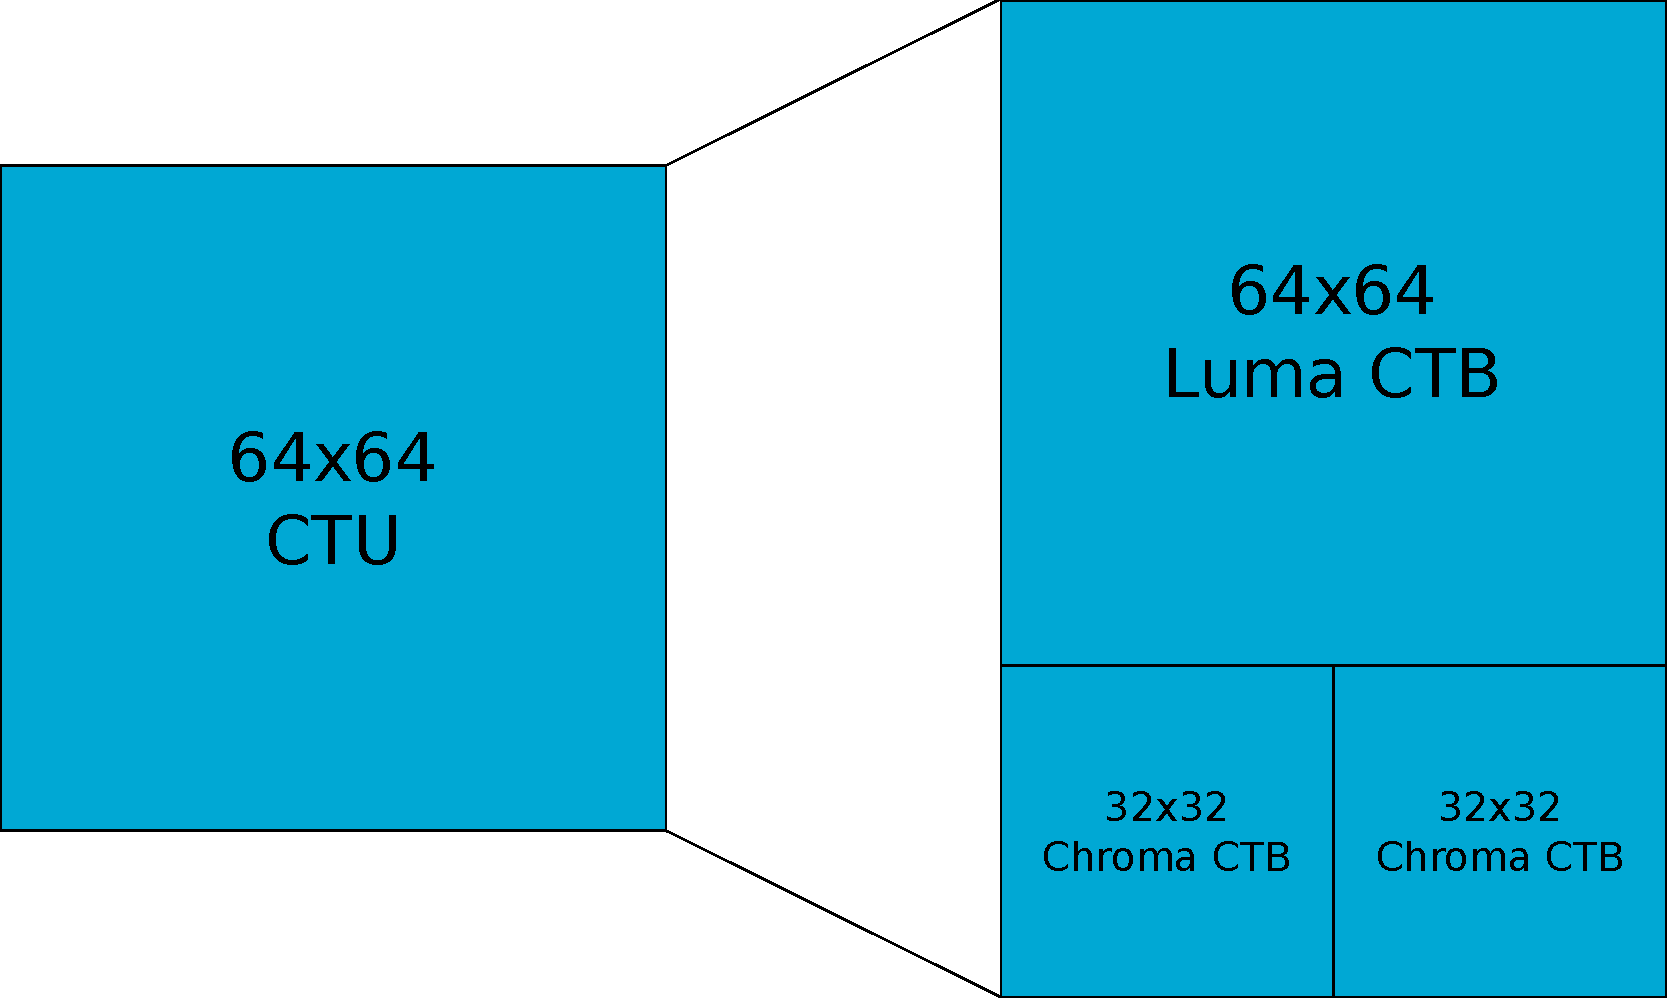
\includegraphics[scale=0.20]{Figures/CTU-CTB}
  \caption{Suddivisione del CTU in CTB}
\end{figure}
// Rivedere questo paragrafo: ovunque viene detto che il CTB è suddiviso \\
// in CU. \\
Il CTB può essere ulteriormente suddiviso in \emph{coding blocks} (CB), che 
sono il punto in cui viene decisa quale tipo di \emph{prediction} utilizzare.
Supponendo di avere un CTB di dimensione 64x64 la suddivisione può essere 
effettuata con CB grandi 64x64, 32x32, 16x16 o 8x8, ottenendo una struttura
detta \emph{quad-tree}, in cui il CTB è suddiviso ricorsivamente. 
Il CB, così come il CTB, consiste ancora nei tre blocchi Y, Cb e 
Cr, che definiscono un \emph{coding unit} (CU), ovverò l'unità in cui viene 
codificato il tipo di predizione. La scelta di quest'ultima è autonoma per ogni 
CU.
\begin{figure}[H]
  \centering
  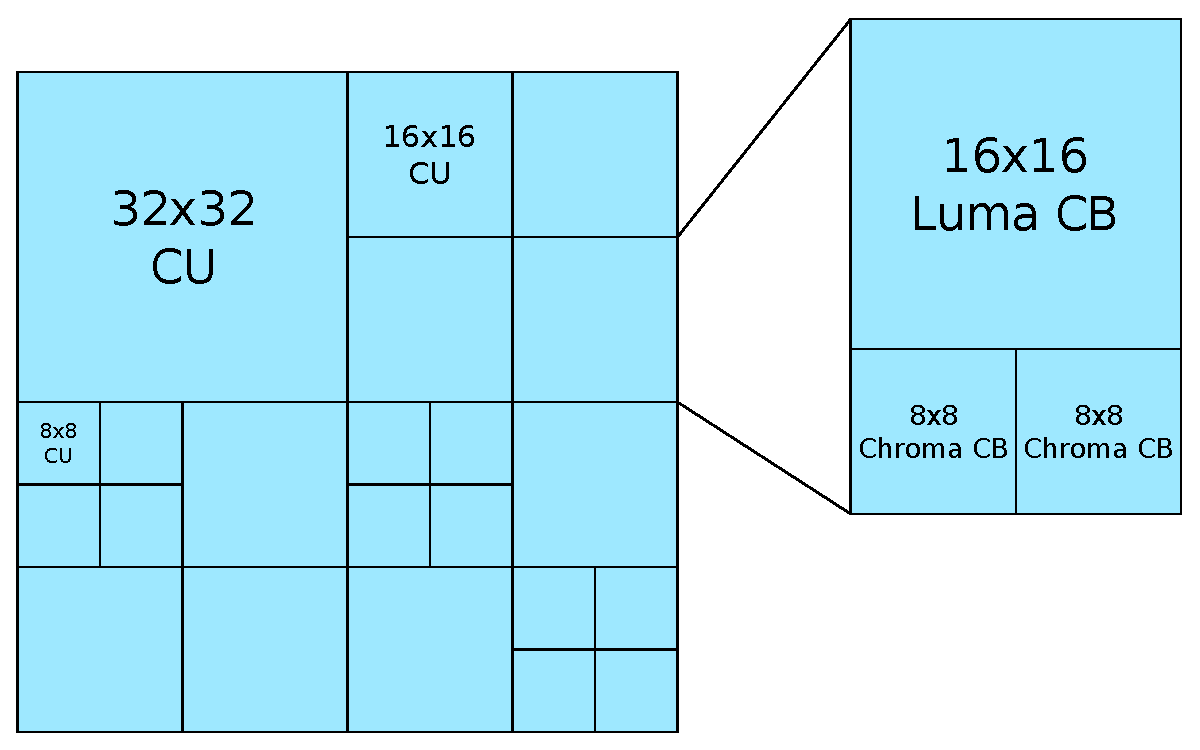
\includegraphics[scale=0.50]{Figures/CTB-CU-CB}
  \caption[Suddivisione del CTB in CU]{Suddivisione di un CTB 64x64 in una 
struttura a \emph{quadtree}}
\end{figure}
In caso ci sia bisogno di una maggiore precisione nella predizione (e.g., 
oggetti minuscoli che si muovono in un CB 8x8) è possibile suddividere i
\emph{coding block} in \emph{prediction block} (PB), che, in caso di 
\emph{inter prediction}, possono non seguire la struttura a \emph{quadtree} dei
blocchi precedenti:
\begin{figure}[H]
  \centering
  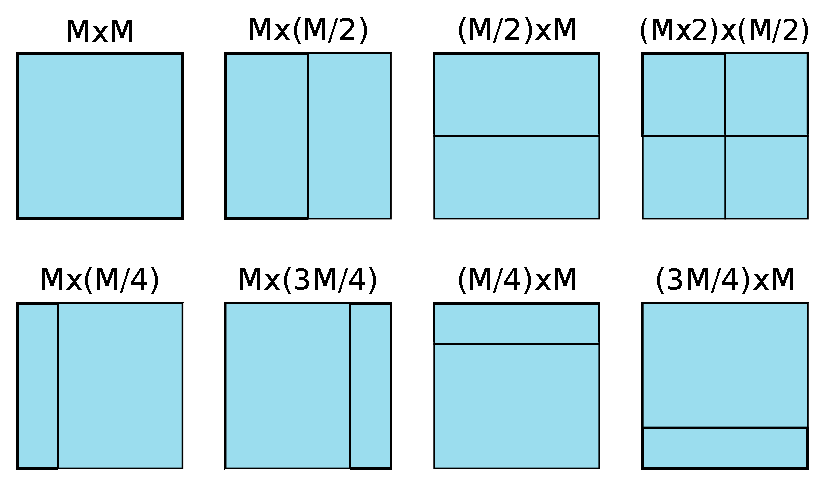
\includegraphics[scale=0.50]{Figures/PB}
  \caption{Possibili strutture di un \emph{prediction block}}
\end{figure}
Un PB definisce una regione che, per effettuare una predizione, utilizza gli 
stessi parametri di movimento: il numero di ipotesi di movimento (che può 
valere uno o due a seconda che si usi l'immagine precedente o quest'ultima 
e le successiva per cercare il blocco che si è mosso) e, per ognuna di queste, 
l'indice dell'immagine di riferimento e il vettore di movimento.
L'insieme dei tre PB, che possiedono lo stesso tipo di suddivisione, 
forma una \emph{prediction unit} (PU).
Per effettuare la codifica del segnale di errore un CB viene suddiviso in 
\emph{transform block}, dando forma ad una struttura a \emph{quadtree} che 
viene chiamata \emph{residual quadtree} (RQT); solitamente la suddivisione 
è mantenuta uguale per i TB Luma e Chroma.
%-------------------------------------------------------------------------------
%	SECTION 2
%-------------------------------------------------------------------------------
\section{Intra prediction}
Su un blocco di campioni contigui che possiedono gli stessi parametri 
predittivi, siano essi CB o PB, verrà eseguita la stessa 
\emph{intra prediction}.
Di quest'ultima esistono due tipologie a seconda delle caratteristiche 
del blocco: in caso di figure e strutture geometriche sarà utilizzata 
la \emph{angular prediction}, viceversa, se la predizione viene eseguita 
su contenuti meno strutturati, sarà eseguita una \emph{planar + DC prediction}. 
In entrambi i casi, la predizione si basa sui campioni contigui (o 
\emph{neighbour}) al blocco che si trovano a sinistra e a destra di 
quest'ultimo.

\paragraph*{Pre-filtering}
Prima di effettuare una delle due predizioni è possibile eseguire uno 
\emph{smoothing filter} sui campioni di riferimento, che dipende dal tipo di 
predizione che verrà successivamente eseguita. Le due possibilità sono le 
seguenti:
\begin{enumerate}
\item Un semplice \emph{lowpass filter} lineare con risposta all'impulso 
[1 2 1]/4 (a)
\item Se la dimensione del TB è 32x32 e i campioni di riferimento sono 
abbastanza ``morbidi'', questi vengono sostituiti con le corrispondenti 
interpolazioni lineari dei cambioni agli estremi (b)
\end{enumerate}

\begin{figure}[H]
  \centering
  \begin{tabular}{cc}
    \subfloat[]{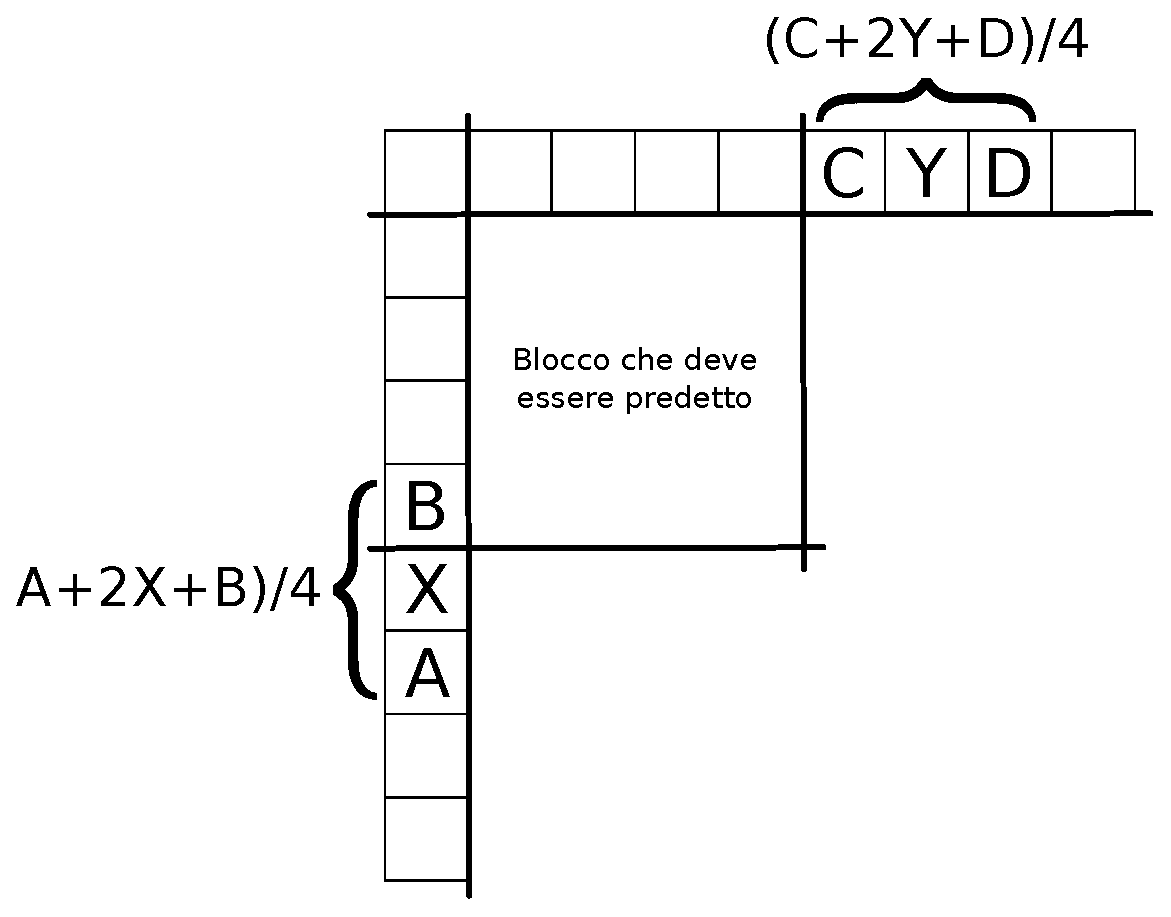
\includegraphics[scale=.35]{Figures/Filtering_a}}
    &
    \subfloat[]{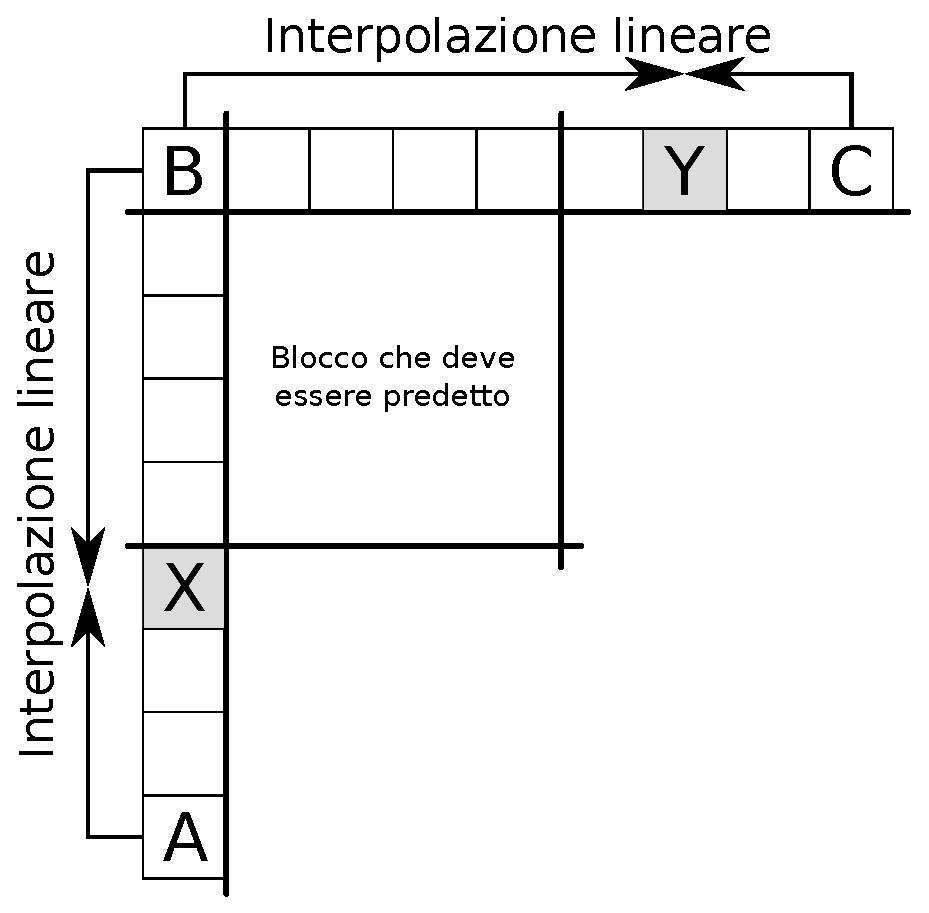
\includegraphics[scale=.35]{Figures/Filtering_b}}
  \end{tabular}
  \caption{I due diversi tipi di \emph{pre-filtering}}
\end{figure}
%-----------------------------------
%       SUBSECTION 1
%-----------------------------------

\subsection{Angular prediction}
Per la predizione angolare l'encoder deve scegliere uno tra 33 possibili angoli:
 questo tipo di predizione stima in modo accurato le strutture direzionali che 
sono tipicamente presenti nelle foto, tra cui le più frequenti risultano essere
 quelle orizzontali e verticali.
Per far fronte a quest'ultima circostanza, H.265 predispone gli angoli in modo 
che siano presenti in numero maggiore intorno alle due direzioni più frequenti;
 il numero totale di angoli e la loro disposizione è il risultato della ricerca 
di un buon \emph{trade-off} tra qualità e complessità computazionale 
dell'encoder.
\\
// Immagine qui
\\
Gli angoli prendono il nome di ``modi predittivi'' (\emph{prediction modes}) e 
il loro raggruppamento è diviso tra orizzontali e verticali.
Nell'immagine di cui sopra si può notare come gli angoli ``orizzontali'' siano 
quelli il cui segmento ha la sua origine in un campione collocato a sinistra, 
mentre l'origine del segmento degli angoli ``verticali'' risiede in un campione 
posizionato in alto.\\
Il parametro angolare $A$ indica la posizione, in termini di campioni, rispetto 
al campione centrale (che ha valore $0$).
Utilizzando il raggruppamento e il parametro $A$ è possibile identificare 
univocamente un modo predittivo; prendendo nuovamente in esame l'immagine la 
sigla $H+2$ corrisponde al modo predittivo 9, la sigla $H-2$ al modo predittivo 
11 e così via.\\
Per effettuare le predizioni dei campioni di un blocco viene prima costruito, 
per comodità, un array che contiene i campioni di riferimento riposizionati 
nell'ordine che risulta più conveniente per il modo predittivo scelto; infatti 
ogni campione $p[x][y]$ da predire viene ottenuto mediante l'interpolazione dei 
due campioni contigui all'interno dell'array di riferimento, con il fattore di 
interpolazione che risulta essere proporzionale all'angolo -o modo predittivo- 
selezionato.
%-----------------------------------
%       SUBSECTION 2
%-----------------------------------

\subsection{DC + Planar prediction }
\paragraph*{DC} La predizione DC prevede un valore costante per tutto il 
blocco, determinato dalla media dei valori dei campioni di riferimento che si 
trovano sopra e a sinistra del blocco.

\paragraph*{Planar} La predizione ``planare'' genera un blocco che presenta 
colori morbidi e privi di discontinuità marcate anche ai bordi. Questo è 
ottenuto tramite una semplice interpolazione, punto per punto, dei campioni di 
riferimento (evidenziati in giallo) con i loro estremi (evidenziati in grigio):
\begin{align*}
p[x][y] = 
%\left
[&\fcolorbox{yellow}{white}{$(N-1-x)*p(-1,y)$}+
  \fcolorbox{black!50}{white}{$(x+1)*p(N,-1)$}+\\
 &\fcolorbox{yellow}{white}{$(N-1-y)*p(x,-1)$}+
  \fcolorbox{black!50}{white}{$(y+1)*p(-1,N)$}+N] \gg log_2(N+1)
%\right]
\end{align*} 
dove $NxN$ è la dimensione del TB.
\\
// Inserire immagine
\\ 
L'immagine mostra come il risultato (c) sia la media di due interpolazioni: una 
orizzontale (a) e una verticale (b).
%-----------------------------------
%       SUBSECTION 3
%-----------------------------------

\subsection{Post-filtering}
Esistono tre casi in cui è necessario eseguire anche un filtraggio successivo, 
tipicamente quelli in cui si presentano brusche discontinuità ai bordi, e sono 
gli \emph{angular mode} esattamente orizzontali e verticali e la 
\emph{DC prediction}.
Il fatto che venga eseguito in sole tre evenienze è determinato dalla volontà 
di limitare la complessità computazionale di fronte a svantaggi che possono 
risultare  marginali, come nel caso delle predizioni diagonali, e dalla ricerca 
di un buon rapporto tra qualità e precedente complessità.
In seguito a test sperimentali è stato notato che le predizioni dei canali 
Chroma risultano sempre relativamente morbide; conseguentemente questo 
filtraggio viene eseguito solo sui canali Luma, e consiste nella modifica dei 
pixel ai bordi all'interno del blocco, secondo le seguenti modalità:
\begin{enumerate}
\item \emph{Angular prediction}, angolo verticale: \\
\begin{align*}
p(0,y)\mathrel{+}=\left(\frac{p*(-1,y)-p*(-1,-1)}{2}\right) 
\forall y \in {[0,N-1]}
\end{align*}

\item \emph{Angular prediction}, angolo orizzontale: \\
\begin{align*}
p(x,0)\mathrel{+}=\left(\frac{p*(x,-1)-p*(-1,-1)}{2}\right) 
\forall x \in {[0,N-1]}
\end{align*}

\item{ \emph{DC prediction}, posto $dcVal$ il valore della posizione: \\
\begin{align*}
p(0,0)=(p*(-1,0)+2dcVal+p*(0,-1)+2)*4
\end{align*}

Con i campioni ai bordi filtrati nel seguente modo:
\begin{align*}
p(x,0)&=(p*(x,-1)+3dcVal+2)*4 \forall y \in {[0,N-1]} \\
p(0,y)&=(p*(-1,y)+3dcVal+2)*4 \forall y \in {[0,N-1]}
\end{align*}

Dove $dcVal \in {[0,1]}$
}
\end{enumerate}

L'immagine seguente mostra un esempio di CTB Luma interamente predetto intra: \\

// Inserire immagine
%-------------------------------------------------------------------------------
%       SECTION 3
%-------------------------------------------------------------------------------

\section{Inter Prediction}
L'\emph{inter prediction} sfrutta la correlazione temporale dei frame per 
ottenere una \emph{motion compensated prediction} (MCP), ovvero un PB predetto 
a partire da PB ``predittori'' che appartegono a frame precedentemente 
decodificati, supponendo che nel PB predetto essi siano traslati: 
\\
// Inserire immagine
\\
Per ogni PB l'encoder ricava un vettore ${(\Delta x,\Delta y,\Delta t)}$ 
chiamato \emph{motion data}, dove ${(\Delta x,\Delta y)}$ è il 
\emph{motion vector} e indica la traslazione compiuta dal PB in questione, 
mentre ${(\Delta t)}$ è l'indice temporale dell'immagine a cui appartiene il PB 
predittore.
È anche possibile effettuare una ``bipredizione'': in questo caso si usano 
due \emph{motion data} ottenendo due MCP di cui viene ricavata la media (che 
può anche essere pesata) per ottenere il risultato, come illustra la figura 
precedente.
\\
Viene inoltre sfruttata la correlazione spaziale (ma sempre legata al tempo) 
dei \emph{motion vector}, basata sulla supposizione che i \emph{motion vector} 
relativi a PB spazialmente vicini non differiscano eccessivamente, eccezion 
fatta per eventuali punti di discontinuità come i cambi di oggetto. È inoltre 
ipotizzata una discreta continuità nel tempo per quanto riguarda i movimenti 
dell'intero \emph{frame}, escludendo variazioni brusche come i cambi di scena.
\\
Tutto questo viene tradotto nel concetto di \emph{motion vector predictor} 
(MVP); invece di trasmettere un \emph{motion vector} per ogni PB l'encoder 
trasmette l'errore o la \emph{motion vector difference} (MVD), tra quello 
predetto a partire da blocchi spazialmente o temporalmente contigui e quello 
normalmente calcolato con $MVD=MV-MP$.
Il decoder riceve la MVD e la sintassi necessaria a determinare il MVP (ovvero 
il tipo di predizione da utilizzare) e può dunque ricavare $MV$ come $MVD+MVP$.
 
Sebbene gli algoritmi che hanno preceduto H.265 (H.264, AVC) possiedano questo 
tipo di predizione, essi si limitano a calcolare $MVP$ come una media dei $MV$ 
vicini spazialmente: questa strategia non è più applicabile in HEVC a causa 
dell'elevata flessibilità delle strutture di predizione.
Il \emph{worst case scenario} presenta 16 $MV$ per lato da tenere in 
considerazione (come mostrato nell'immagine successiva), che porterebbe a 
complessità di codifica troppo elevate.

\begin{figure}[H]
  \captionsetup{justification=raggedright}
  \centering
  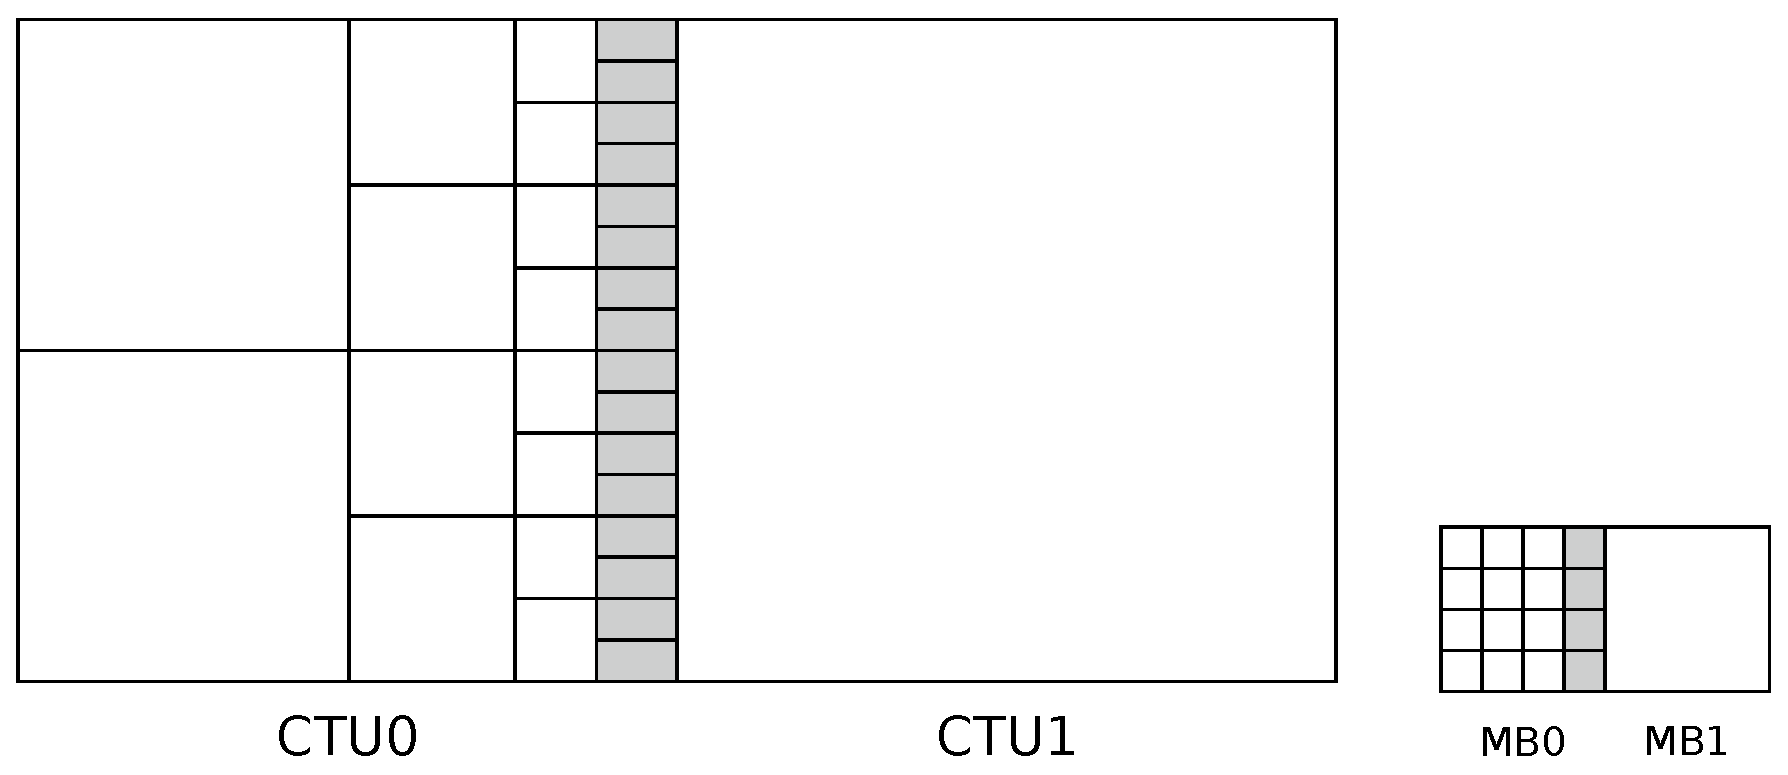
\includegraphics[scale=0.45]{Figures/Inter_pred_2}
    \caption[Numero massimo di \emph{motion vector} in H.265 e H.264]
    {Numero massimo di \emph{motion vector} in H.265 (a sinistra) e H.264 \\
      (a destra). CTU0 possiede 16 PB Luma 8x4 contigui a CTU1 che è composto da
      un solo PB Luma 64x64. MB0 (\emph{Macro Block)} contiene quattro 
      partizioni di predizione 4x4 affiancate a MB1 che consta di una 
      partizione 16x16. }
\end{figure}

H.265 mette a disposizione un algoritmo per la costruzione di vettori 
\emph{candidate MVP} chiamato \emph{advanced motion vector prediction} (AMVP), 
ottenuto in seguito ad esperimenti esaustivi volti a trovare oredizioni che 
minimizzassero la complessità di codifica pur mantenendo buoni livelli di 
predizione (i.e., bassa entropia del segnale di errore MVD).\\
Una parte della sintassi di HEVC serve a comunicare al decoder quale MVP 
utilizzare tra quelli candidati, che sono due e scelti nei modi seguenti:
\begin{itemize}
\item Due \emph{spatial candidate} che derivano da cinque blocchi spazialmente 
vicini;
\item Viene tenuto come riserva un \emph{temporal candidate} derivato da due 
blocchi co-locati e temporalmente vicini:
\begin{itemize}
\item Nel caso che i due \emph{spatial candidate} siano uguali, o se uno di loro
 non sia disponibile, i due vettori candidati saranno uno spaziale e uno 
temporale;

\item Se entrambi i candidati spaziali non fossero disponibili, verrà 
considerato il vettore candidato temporale di riserva ed uno 
\emph{zero motion vector};

\item Nell'eventualità che sia i candidati spaziali sia i candidati temporali 
non siano disponibili, entrambi i candidati saranno \emph{zero motion vector}.
\end{itemize}
\end{itemize}

Gli \emph{spatial candidate} sono ottenuti prendendo in considerazione cinque 
blocchi spazialmente vicini suddivisi in due gruppi: il gruppo A contenente i 
due blocchi in basso a sinistra rispetto a quello che si vuole predire, il 
gruppo B con al suo interno tre blocchi in alto.
Generalmente, se i vettori dei blocchi considerati sono ricondicibili allo 
stesso \emph{reference id} (l'indice dell'immagine a cui fanno 
riferimento) di quello del blocco che si vuole predire, tali vettori saranno 
MVP.
Viceversa, MVP sarà il vettore scalato secondo una formula che dipende dalla 
differenza temporale dei \emph{reference id}.
Non sono invece presi in considerazione blocchi a destra o in basso dal 
momento che tali PB non sono ancora stati decodificati e non sono disponibili 
al decoder per la predizione.
\\
Per quanto concerne il \emph{temporal candidate} si lavora su una immagine 
co-locata e temporalmente vicina della quale, in fase di decodifica, si 
possiedono tutte le informazioni (ovvero un frame già decodificato); diversi 
esperimenti hanno dimostrato che i blocchi da prendere in considerazione sono 
due: quello al centro e quello in basso a destra rispettivamente alla posizione 
del blocco che si vuole predire.
Specificamente il vettore viene predetto utilizzando sempre il blocco in basso 
a destra, salvo la mancanza di disponibilità d quest'ultimo; ciò significa che 
esso risiede fuori dai bordi dell'immagine o viola vincoli imposti per motivi 
di memoria.
\newline \\
Infine HEVC risolve un problema legato alla struttura di suddivisione delle 
immagini \emph{quadtree}: quest'ultime permettono una grande flessibilità 
delle dimensioni dei blocchi con un basso costo di \emph{overhead} in termini 
di \emph{bit rate}. Per l'\emph{inter prediction} la struttura a \emph{quadtree}
 permette di suddividere minuziosamente quelle parti di immagine dhe presentano 
bruschi movimenti rispetto alle parti più statiche che non richiedono una 
grande informazione di movimento. Questo tipo di raggruppamento, tuttavia, 
origina facilmente bordi ineffettivi (\emph{over segmentation}); HEVC dispone 
di un  algoritmo di \emph{block merging} che consente di raggruppare PB con 
uguali parametri di predizione in modo da trasmetterne una sola copia.
\\
Nell'esempio mostrato dall'immagine seguente la parte a) è l'immagine 
originale, b) è l'immagine scomposta in PB secondo la struttura a 
\emph{quadtree} mentre c) mostra il risultato del \emph{block merging}.
\\
// Inserire immagine 
\\
%-------------------------------------------------------------------------------
%       SECTION 4
%-------------------------------------------------------------------------------

\section{Transform and Quantization}
Nel \emph{block-based video coding} i segnali di errore residui che derivano 
dalle predizioni intra o inter vengono trasformati e quantizzati prima di 
essere trasmessi.
Più nel dettaglio, un'immagine è suddivisa in blocchi quadrati di dimensione $NxN$, dove $N=2^M$ con $M \in \mathbb{N}$. Per ogni blocco esisterà un blocco 
residuo $U$ che verrà trasformato e quantizzato. \\
L'immagine mostra il percorso dei dati durante la fase di encoding (a) e 
di decoding (b):
\begin{figure}[H]
  \centering
  \begin{tabular}{cc}
    \subfloat[]{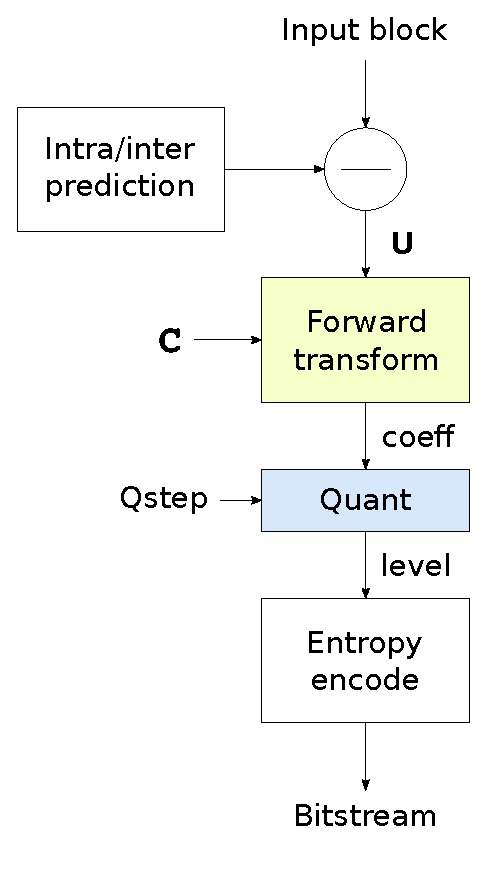
\includegraphics[scale=.66]{Figures/Transf_and_quant_a}}
    &\qquad
    \subfloat[]{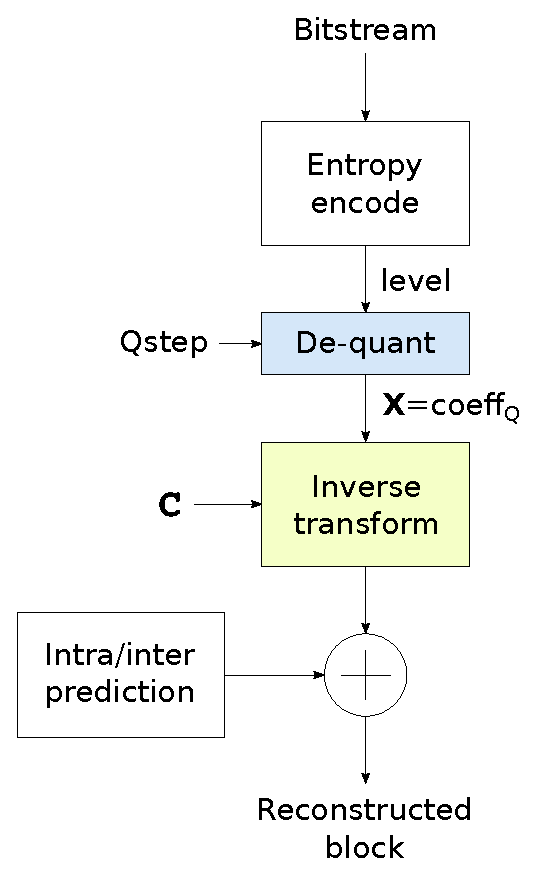
\includegraphics[scale=.66]{Figures/Transf_and_quant_b}}
  \end{tabular}
  \caption{\emph{Data flow} di encoding e decoding.}
\end{figure}
\subsection{Transform}
Tipicamente le trasformate sono delle matrici costruite in modo tale che, in 
assenza di quantizzazione, sommando trasformata e trasformata inversa si 
ottenga un risultato praticamente lossless.
HEVC utilizza due tipologie di trasformate, ovvero quelle derivate dalla DCT e
quelle derivate dalla DST; fornisce inoltre delle matrici precostruite per 
eseguire l'antitrasformata DCT e DST per tutte le possibili dimensioni dei 
blocchi: $4x4$, $8x8$, $16x16$ e $32x32$.
Queste matrici contengono approssimazioni ad interi con precisione finita dei 
coefficienti di trasformazione DCT-II; questo sistema riduce di molto la 
complessità di encoder e decoder, e risolve un problema che era presente in 
H.261, ovvero la deriva dovuta a lievi disallineamenti nella rappresentazione 
fixed point dei coefficienti tra la matrice di trasformazione, costruita 
arbitrariamente dal'implementatore dell'encoder, e quella di antitrasformazione 
fornita dallo standard. \\
Errori di questo tipo si ripercuotono amplificati in ogni immagine successiva, 
costringendo a dover trovare un modo di ovviare al problema (il sopracitato 
H.261 costringeva un aggiornamento periodico del segnale che consisteva in una 
immagine codificata interamente intra).
\subsection{Quantization}
Con ``quantizzazione'' si intende la divisione dei valori trasformati 
utilizzando un passo di quantizzazione $Q_s$ (\emph{quantization step}) definito
 attraverso il parametro di quantizzazione $Q_p$ come segue:
\begin{align*}
Q_s = \left(2^{\frac{1}{6}}\right)^{(Q_p-4)}
\end{align*}
Dalla formula si può notare come una variazione di $1$ per $Q_p$ si traduca in 
una moltiplicazione di $Q_s$ per un fattore $2^{\frac{1}{6}}\approx 1.12$, ovvero 
nell'incremento di $Q_s$ del $12\%$. Una variazione di $6$ si traduce in un 
raddoppiamento di $Q_s$ \\
Si può anche eseguire una quantizzazione \emph{frequency dependent} specificando
 una matrice $w$ con un valore di quantizzazione per ogni frequenza, con un 
risultato che risulta il seguente:
\begin{align*}
q[x][y] = \frac{tc[x][y]}{q[x][y]*Q_s}+offset
\end{align*}
dove $tc$ sono i coefficienti trasformati. \\
Si ottiene una compressione in quanto i valori, una volta quantizzati, verranno 
arrotondati all'intero più vicino. Il fine è quello di portare a 0 il maggior 
numero possibile di coefficienti in modo che la codifica successiva (marcata 
come \emph{Entropy encode}) sia in grado di comprimere al meglio la sequenza in 
uscita; dividendo un intero per un numero più grande il risultato sarà più 
vicino a zero. Tipicamente le matrici di quantizzazione possiedono valori più 
grandi alle basse frequenze e viceversa alle alte, perché il contenuto utile 
per il sistema visivo umano è concentrato alle basse frequenze.

%-------------------------------------------------------------------------------
%       SECTION 5
%-------------------------------------------------------------------------------

\section{In-Loop Filters}
Lo standard ibrido di codifica HEVC scompone i frame attraverso una struttura a 
blocchi per effettuare la compressione; questa suddivisione porta spesso alla 
comparsa di artefatti che danno alle sequenze video un'aspetto quadrettato, 
peggiorandone la qualità visiva. Un esempio tipico di causa della discontinuità 
tra i blocchi è la predizione inter di due blocchi contigui che nel frame
 di riferimento erano distanti, oppure anche la codifica di due blocchi contigui
 con modalità predittive differenti (due intra diversi, una inter e una intra, 
etc.). Per porre rimedio a questi artefatti lo standard HEVC specifica due 
filtraggi: il \emph{deblocking filter} e il \emph{sample adaptive offset} (SAO).
\\ \\
Questi filtraggi sono chiamati \emph{in-loop filters} perché vengono eseguiti 
all'interno dei cicli di encoding/decoding, e i risultati vengono utilizzati 
nei cicli successivi oltre che durante la visualizzazione delle sequenze 
decodificate; in questo modo si trae vantaggio da questa procedura anche durante
 il decoding dei frame successivi, preché le predizioni inter vengono effettuate
 a valle di frame reference di maggiore qualità.
\\ \\
Il \emph{deblocking filter} si occupa di smussare i confini tra due blocchi in 
cui è presente una discontinuità, cercando di lavorare solo su quelle 
introdotte durante la compressione e non quelle originariamente presenti nella 
sequenza. \\
Il SAO, invece, si occupa di ridurre gli artefatti dovuti a trasformazioni e 
quantizzazioni grossolane (chiamati \emph{ringing artifacts}), ed opera 
sull'output del \emph{deblocking filter} in cascata. \\
Visto che i due filtraggi operano su due artefatti diversi, i loro benefici 
sono additivi se eseguiti insieme.
\subsection{Deblocking Filter}
Il \emph{deblocking filter} si applica solo ai confini tra blocchi di tipo CU, 
PU o TU e non al loro interno; durante la codifica  l'encoder considera gruppi 
di quattro vettori di campioni perpendicolari ai confini dei blocchi. 
Specificamente l'encoder esegue alcuni controlli sul primo e sul quarto vettore 
per decidere:
\begin{itemize}
\item Se eseguire il filtraggio o meno;
\item In caso positivo quale filtraggio applicare tra \textbf{normal} e 
\textbf{strong}.
\end{itemize}
Questi semplici controlli misurano un indice di distorsione dei vettori di 
campioni rispetto ad una delle funzioni continue più semplici, ovvero una rampa 
che attraversa il confine \textbf{/*(di che cosa?)*/}. Se questo indice supera 
una certa soglia, che dipende dal passo di quantizzazione $Q_p$ secondo una 
\emph{look-up table}, si esegue il filtraggio.

\begin{figure}[H]
  \captionsetup{justification=raggedright}
  \centering
  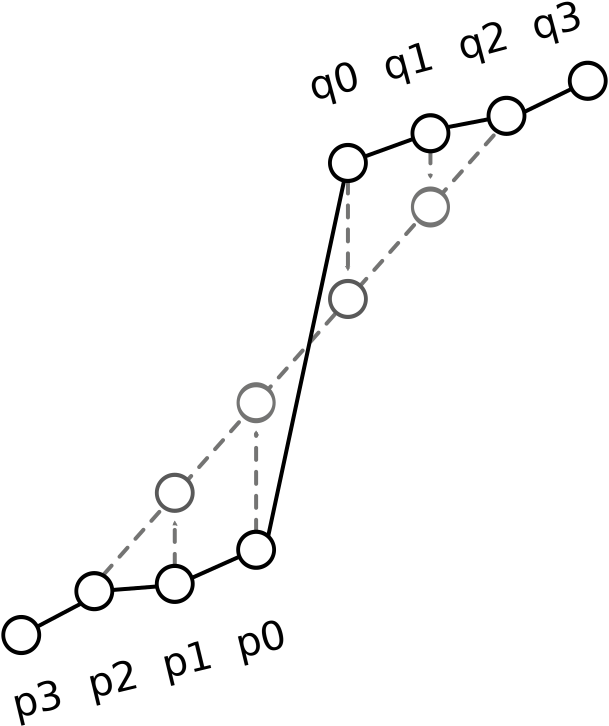
\includegraphics[scale=0.45]{Figures/Deblocking_filter}
    \caption[Filtraggio \emph{deblocking} di tipo \textbf{normal}]
    {Filtraggio \emph{deblocking} di tipo \textbf{normal}: la linea nera mostra
      il confine originale del blocco, la linea grigia tratteggiata quello 
      nuovo}
\end{figure}

L'immagine mostra il risultato di un filtraggio \textbf{normal} eseguito su un 
vettore di 8 campioni, con questi ultimi appartenenti a due blocchi confinanti 
chiamati $P$ e $Q$. \\
In generale, un filtraggio \textbf{normal} può arrivare a modificare fino a due
campioni per lato avvicinandoli alla rampa, come accade nell'immagine.
Il filtraggio \textbf{strong} viene utilizzato nelle aree che racchiudono 
contenuti a bassa frequenza, ovverosia quelle in cui il sistema visivo umano è 
più sensibile alle discontinuità, e consiste in un filtraggio lineare lowpass 
che comprende tre campioni per lato.
\\ \\
Il filtraggio \emph{deblocking} descritto interessa solamente il canale luma, 
dal momento che per i canali chroma si opera un filtraggio analogo ma più 
grossolano, in cui vengono eseguiti molti meno controlli e vengono considerati 
meno campioni: ciò permette di ridurre la complessità dell'encoder a fronte di 
una bassa perdita di qualità, sempre considerando il fatto che i canali chroma 
sono meno importanti per il sistema visivo umano.
\subsection{Sample Adaptive Offset - SAO}
 
%\input{Chapters/Chapter5} 
%\input{Chapters/Chapter6} 
%\input{Chapters/Chapter7} 

%----------------------------------------------------------------------------------------
%	THESIS CONTENT - APPENDICES
%----------------------------------------------------------------------------------------

\addtocontents{toc}{\vspace{2em}} % Add a gap in the Contents, for aesthetics

\appendix % Cue to tell LaTeX that the following 'chapters' are Appendices

% Include the appendices of the thesis as separate files from the Appendices folder
% Uncomment the lines as you write the Appendices

% Appendix A

\chapter{Appendix Title Here} % Main appendix title

\label{AppendixA} % For referencing this appendix elsewhere, use \ref{AppendixA}

\lhead{Appendix A. \emph{Appendix Title Here}} % This is for the header on each page - perhaps a shortened title

Write your Appendix content here.
%\input{Appendices/AppendixB}
%\input{Appendices/AppendixC}

\addtocontents{toc}{\vspace{2em}} % Add a gap in the Contents, for aesthetics

\backmatter

%----------------------------------------------------------------------------------------
%	BIBLIOGRAPHY
%----------------------------------------------------------------------------------------

\label{Bibliography}

\lhead{\emph{Bibliography}} % Change the page header to say "Bibliography"

\bibliographystyle{unsrtnat} % Use the "unsrtnat" BibTeX style for formatting the Bibliography

\bibliography{Bibliography} % The references (bibliography) information are stored in the file named "Bibliography.bib"

\end{document}